\newchap{Technical Background}
\label{chap:tech-background}
This chapter presents the technical background that is needed for this thesis. It explores everything around automated models that can be used to create phonetic transcriptions. I will first set the basis and dive into evaluation metrics and general architectures and frameworks that are commonly used and then present current state-of-the-art models. Table \ref{tab:sota} shows the state-of-the-art models for \ac{g2p} modelling.

\tab{tab:sota}{This table presents the state-of-the-art \ac{g2p} models. Models that are important for this thesis will be explained in more detail. The language code in parenthesis is the code used in the respective paper.}{
\begin{tabularx}{\textwidth}{
| 	>{\raggedright\arraybackslash}l | 
	>{\raggedright\arraybackslash}l | 
	X | 
	>{\raggedright\arraybackslash}r |}
\hline
\textbf{Author} & \textbf{Model Architecture} & \textbf{ISO 639-3} & \textbf{WER} \\
\hline
\hline
\multirow[t]{11}{0.14\textwidth}{SIG21: \citet{Clematide&Makarov.2021} \\
\vspace{0.5cm}
\href{https://aclanthology.org/2021.sigmorphon-1.17/}{\underline{Link}}}& \multirow[t]{11}{0.5\textwidth}{CLUZH models 1-7. LSTM-based neural transducer with pointer network-like monotonic hard attention trained with imitation learning. All models 1-7 are majority-vote ensembles with different number of models (5-30) and different inputs (characters or segments). \\
\vspace{0.5cm}
Achieved good results in nld (14.7), ice (10), jpn (5.0), fra (7.5) and vie (2.0) but not better than SIG20.

}& \multicolumn{2}{c|}{medium (10,000 pairs)} \\\cline{3-4}
& & hye (arm\_e) & 6.4 \\
& & hun & 1.0 \\
& & kat (geo) & 0.0 \\
& & kor & 16.2 \\\cline{3-4}
& & \multicolumn{2}{c|}{low (800 train pairs)} \\\cline{3-4}
& & ell (gre) & 20 \\
& & ady & 22 \\
& & lav & 49 \\
& & mlt\_ltn & 12 \\
& & cym (wel\_sw) & 10 \\
\hline
\multirow[t]{4}{0.14\textwidth}{SIG21: \citet{lo-nicolai-2021-linguistic} \\
\vspace{0.5cm}
\href{https://aclanthology.org/2021.sigmorphon-1.15/}{\underline{Link}}}& \multirow[t]{4}{0.5\textwidth}{UBC-2 outperforms the baseline. They analysed the errors of the baseline and extend it by adding penalties for wrong vowels and wrong diacritics. Errors on vowels actually decreased. Best macro average (low -resource).
}& ady & 22 \\
& & khm & 28 \\
& & lav & 49 \\
& & slv & 47 \\
\hline
\multirow[t]{4}{0.14\textwidth}{SIG21: \citet{gautam.2021} \\
\vspace{0.5cm}
\href{https://aclanthology.org/2021.sigmorphon-1.16/}{\underline{Link}}}& \multirow[t]{4}{0.5\textwidth}{Dialpad-1: Majority-vote ensemble consisting of three different public models (weighted \ac{fst}, joint-sequence model trained with \ac{em} and a neural \ac{s2s}), two \ac{s2s} variants (LSTM and transformer) and two baseline variations. 
}& \multicolumn{2}{c|}{high (32.800 train pairs)} \\\cline{3-4}
& & eng (eng\_us)  &  37.43 \\
& &   &   \\
& &   &   \\
\hline
\multirow[t]{5}{0.14\textwidth}{SIG20: \citet{peters-martins-2020-one} \\
\vspace{0.5cm}
\href{https://aclanthology.org/2020.sigmorphon-1.4/}{\underline{Link}}}& \multirow[t]{5}{0.5\textwidth}{DeepSPIN-2,-3,-4: Transformer- or LSTM-based enc-dec \ac{s2s} models with sparse attention. Add language embedding to enc or dec states instead of language token.
}& \multicolumn{2}{c|}{3.600 train pairs} \\\cline{3-4}
& & jpn (jpn\_hira) & 4.89 \\
& & fra (fre) & 5.11 \\
& & rum & 9.78  \\
& & vie  & 0.89  \\
\hline
\multirow[t]{4}{0.14\textwidth}{SIG20: \citet{yu-etal-2020} \\
\vspace{0.2cm}
\href{https://aclanthology.org/2020.sigmorphon-1.5/}{\underline{Link}}}& \multirow[t]{4}{0.5\textwidth}{IMS: Self training ensemble of one n-gram-based \ac{fst} and 3 \ac{s2s} (vanilla with attention, hard monotonic attention with pointer, hybrid of hard monotonic attention and tagging model). 
}& hin &  5.11 \\
& & nld (dut) & 13.56  \\
& &   &   \\
& &   &   \\
\hline
\end{tabularx}}{SOTA \ac{g2p} models}

\section{Evaluation metrics}
The evaluation of phonetic transcriptions depends on whether the system output and the reference are sentences or single words, i.e. character sequences. The most common metric to evaluate the former is the \ac{wer}. The lower the score, the better the model. If the \ac{wer} is 0, this means that the texts are exactly the same. The following formula is used to calculate \ac{wer}:    

\begin{equation}
\label{eq:wer}
WER = \frac{S+I+D}{N}
\end{equation} 


In equation \ref{eq:wer} the $S$ stands for substitution, $I$ for insertion, $D$ for deletion and $N$ denotes the total number of words in the reference sequence. Those numbers can be calculated by using an algorithm to get the edit distance. The idea behind the score is that we can capture the cost that it takes to transform the system output into the reference phoneme sequence. If you want the percentage, the number needs to be multiplied with $100$. Note that the \ac{wer} can be more than $100$\%. This happens if, for example, the are a lot of additional insertions or deletions in the system text. If the system output and reference are character sequences, the score is called \acf{cer}. It is calculated in the exact same way as the \ac{wer}, but instead of words everything is calculated on character basis. In the phonetic transcriptions setting, the \ac{cer} is typically replaced by the \acf{per} to match the correct terminology. The calculations are not changed. In a multilingual setting, it is sometimes necessary to have a score for the entire system covering more than one language. In such cases it is custom to use a macro-averaged \ac{wer} or \ac{cer}. This means that the sum of the scores for each language is divided by the number of languages \citep{Leung.2021}.

In the case of \ac{g2p} conversion, the \ac{wer} actually just reflects the rate of wrongly predicted words, as one sequence consists of only one word. 


\section{Automated phonetic transcription}
\label{model_theory}
In this section I set the stage for understanding the technical background of \ac{g2p} models. Today's technologies allow to build models that create phonetic transcriptions automatically given an original text. There are several approaches which I will discuss below. Creating phonetic transcriptions is essentially a \acf{s2s} task. Like other \ac{nlp} tasks its goal is to transform a sequence of characters into another sequence of characters. In particular, it is very similar to machine translation which is such a task as well \citep{Rao2015GraphemetophonemeCU}. In the present case, the input sequence is a sequence of graphemes. These can look very differently depending on the script (see section \ref{writing-sys}). The output sequence is a sequence of phonemes\myfootnote{Please refer to section \ref{phonology} in order to understand the terminological implications of  phoneme. As it is common in research, I will stick to the term \textit{phoneme} although strictly speaking it is not always correct. Phoneme in this case just refers to any symbol that is used to represent a sound.}. This process is typically referred to as \ac{g2p}. There are a few problems and characteristics of the \ac{g2p} task that are important:

\begin{itemize}
\item The input and output sequences are not always of the same length. It is difficult to align input and output. Not all systems rely on aligning input and output but often it is needed to analyse the results (for example to create confusion matrices). 
\item Due to the open-vocabulary situation and the impossibility to cover all possible words, all systems must be able to deal with rare and unseen words \citep{Rao2015GraphemetophonemeCU, ney-joint-sequence2008}. 
\item Most of the research done in this area is limited to the English language. This is not uncommon in \ac{nlp} research. The availability of English data resources and the unavailability and struggles to find data in other languages heavily influences this research. \citet{Ashby&Bartley.2021} report that the \acs{sigm} (\acl{sigm}) \ac{g2p} tasks in 2020 and 2021 are the first attempt to tackle multilingual \ac{g2p}.
\end{itemize}

In the following, I explain the most important model types. Often, those different types are used in combination as the different models have different advantages which can be used very well in combination. 

\subsection{Look-up dictionary} The simplest version of a \ac{g2p} model is a look-up table where a grapheme sequence is stored together with its phonetic transcription. Such a dictionary is expensive to create and needs a lot of storage and has a very limited coverage. Although such a system is no longer useful on its own it can still be used in addition to other, for example, statistical models \citep{ney-joint-sequence2008}.

\subsection{Rule-based models}
The first systems to create phonetic transcriptions of text were rule-based systems. Although rule-based systems are outperformed by more recent neural models \citep{Ashby&Bartley.2021, gorman-etal-2020-sigmorphon}, I will introduce them as they were an important step towards \ac{g2p} modelling. Additionally, rule-based models can be used together with other models to reach a better performance. Rule-based transcriptions models are built using linguistic pronunciation rules. In order to be able to create such a system, one needs to collect pronunciation rules first. While there are only few languages where such rules are ready and available for the general public there are many languages where those rules need to be created first. In order to create the rules in the first place, a lot of linguistic expertise is needed. Apart from this initial effort to create the rules, a problem with rule-based approaches is the maintenance of the systems. To maintain the system, experts need to keep track of language change which is time consuming and expensive. Most languages are irregular in their pronunciation and those irregularities need to be tracked as well. Another drawback of such systems is that they might fail when presented with unseen or rare words \citep{ney-joint-sequence2008}. Many earlier systems published considered only one language and were not multilingual (see e.g. \citet{rule-based2009}). 

\subparagraph{Epitran} Epitran is an example of a relatively new rule-based system. It makes use of the fact that there are languages that are more or less regularly pronounced and presents a rule-based system for \ac{g2p} conversion for mostly low-resource languages. The system has the ability to provide a solution for every possible word and is consistent within its transcriptions. Epitran for all languages except English and traditional Chinese works with a map file that allows to map graphemes to phonemes. Additional pre- or post-processing can be applied that follow context specific rules \citep{mortensen-etal-2018-epitran}.


\subsection{N-gram Models / Statistical models}
N-gram models, statistical models or joint-sequence models were used before neural models took over the field. These are sometimes referred to as traditional models. One reason why they were outperformed by neural models is that it is necessary to construct alignments between grapheme and phonemes. This is needed because one grapheme can be realized as multiple phonemes or vice versa. It is not possible to simply have a one-to-one alignment. Joint-sequence models were often used with different versions of the \acf{em} algorithm \citep{lo-nicolai-2021-linguistic}. The main intuition about those models is that they, in some way or other, try to statistically model the relationship between graphemes and phonemes. Typically, those models consist of two parts: first an alignment model. Second, a model that captures the relationship between graphemes and phonemes using clearly defined statistical methods. A very common model is the joint-sequence model.

\subparagraph{Joint-sequence model} The term \textit{joint-sequence} hints already at the underlying architecture of those models: the idea is to process \textit{joint} sequences of input and output symbols. In order to do that they must be aligned. We can then concatenate those alignments, which means to concatenate the grapheme and the phoneme which it is mapped to, and receive what is called a graphone. Using the concept of \ac{fst}, we can build a model. \acp{fst} are similar to finite-state automatons. But instead of just telling whether a certain sequence belongs to a certain language (which is pattern matching), they can output none or many symbols at every step as well. This means that in the process of iterating over the sequence, they produce another sequence. Knowing that, it is easily understandable that this works well for our given \ac{g2p} task. The idea is now, that we model the joint-probability of the input graphemes and output phonemes or rather our graphones. Doing this we can use the \ac{em} algorithm to find a mapping of graphemes to phonemes that is most probable. As those graphones consist of n-grams of both the input and output sequence, they themselves can be considered a n-grams which is why those models are sometimes referred to as n-gram models \citep{ney-joint-sequence2008, lo-nicolai-2021-linguistic}.

\subsection{Neural models}
Neural G2P models have been reported to outperform most other models \citep{Lee&Ashby.2020}. Many researchers experiment with different variants of LSTM models \citep{Lee&Ashby.2020, hammond-2021-data, gautam.2021, Rao2015GraphemetophonemeCU}. But there are also other models that have been used. The most important of those will be introduced in the following.

\subparagraph{Sequence-to-sequence}
\ac{s2s} is not a model type as such but rather an architecture. \ac{s2s} models include an encoder and a decoder or more than one of each depending on the exact implementation. Both encoder and decoder can be the same model type or different ones but all of them are \acp{rnn} or some variant of it. The output of the (last) encoder \ac{rnn} is used as input for the decoder \ac{rnn}. What makes such a model architecture powerful is that they can map an input sequence to a output sequence of a different length and different type. 
Generally, there is a difference between models that assume conditional independence between each output step (e.g. Hidden Markov Models) and there are models that do not make this assumption but condition the current output on the entire sequence before. Depending on what model type is used as encoder or decoder considering the entire preceding input can get tricky if the input sequence is really long. This is true especially for \ac{rnn} models. Apart form that, \ac{s2s} models have to wait until the full input sequence is processed before they can start decoding. This does not work well for input that gets continuously longer \citep{Kostadinov.2019, DBLP:journals/corr/SutskeverVL14}. 

\subparagraph{RNN}
The important intuition about \acp{rnn} is that they process each unit of an input sequence one unit at a time. In our case, we can think of one unit as one grapheme in the input sequence. Instead of only outputting something at each time step, a hidden representation is passed on to be processed in the next time step. This sequential processing is crucial as it means that each unit gets information about the units preceding it. This makes sure that information about the preceding context is included. The output of such an \ac{rnn} is therefore a manipulated version of the input sequence of the same length.
A special kind of \ac{rnn} is the LSTM. LSTM means long short-term memory. As their name suggests they include what we could call a memory. Instead of just adding some representation of the preceding units at each time step, LSTMs can more flexibly decide what information is added and what information should be forgotten \citep{Olah.29.01.2022, Kostadinov.2017}.
Many earlier neural LSTM models use a connectionist temporal classification layer to include alignment information \citep{lo-nicolai-2021-linguistic}. This is a special methodology that can deal with n-to-m alignments which is the case in \ac{g2p} modelling.

\subparagraph{Transformer}
Transformers are \ac{s2s} models as well. A central concept and what makes transformers powerful models is their self-attention mechanism. Also, they can process the entire input sequence in one go such that each unit is processed by a separate part of the model instead of just using the same cell for every unit. This allows to have dependencies between the different input units which means that we can model any dependencies within a sentence or a grapheme sequence. This is the reason why we call it \textit{self}-attention as the attention is focused on other parts of the input sequence, but still on the sequence itself \citep{Alammar.03.01.2022}.

\subparagraph{Neural Transducer}
Neural transducers, as presented by \citet{jaitly2016neural}, extend previously used \ac{s2s} models. They can treat more arriving input without having to redo the entire calculation for the entire updated sequence. At each time step, the neural transducer can output zero to many output symbols. 


\begin{landscape}

\thispagestyle{empty}
\begin{figure}[h]
\vspace*{-2.8cm}
    \begin{center}
    \hspace*{-2cm}
      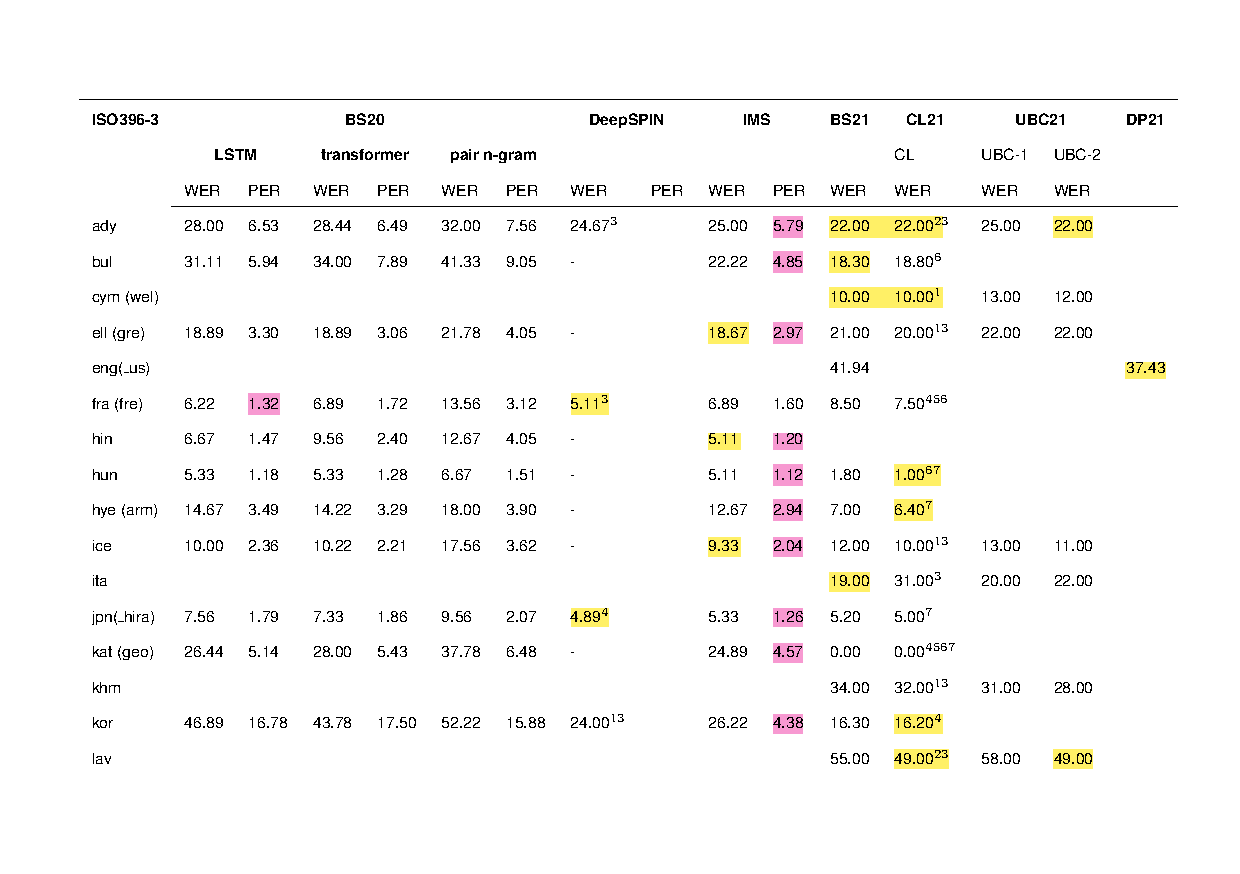
\includegraphics[page=1,width=1.1\linewidth]{SOTA.pdf}
    \end{center}
  \end{figure}
 \end{landscape}
 
\begin{landscape}
\begin{figure}[h]
  \thispagestyle{empty}
\vspace*{-2.8cm}
    \begin{center}
    \hspace*{-2cm}
      \includegraphics[page=2,width=1.1\linewidth]{SOTA.pdf}
    \end{center}
    \stepcounter{myfigure}
    \vspace*{-1.5cm}
    \caption[State-of-the-art models]{The table lists the SOTA models from the SIGMORPHON tasks in 2020 and 2021.}
    \label{fig:sota_table_long}
  \end{figure}
 \end{landscape}
 
\section{State-of-the-art G2P models}
\label{section:sig}
As I have to decide what model I will use to train on my language set, I will now have a look at the state-of-the-art models that can be used for \ac{g2p} conversion.  
The \ac{sigm} \citep{Sigmorphon.2021} regularly organizes shared tasks concerned with morphology and phonology. For the years 2020 and 2021 they organized a \ac{g2p} conversion task \citep{Ashby&Bartley.2021, gorman-etal-2020-sigmorphon}. The tasks represent a first attempt at creating benchmarks for multilingual \ac{g2p} conversion. Although there is other research on \ac{g2p}, many recent publications have been made within the \ac{sigm} shared tasks. 
In the next sections, I will summarize the results and insights from \ac{g2p} research.

\subsection{Model architectures}
An essential part of \ac{g2p} modelling is the actual model. In section \ref{model_theory} I explained the most important theoretical basics. For this part here, I familiarized myself a bit more with works well in practice and what some concrete problems are. 

\subparagraph{Ensembles}
Many models that are used and achieve peek performance for \ac{g2p} modelling are ensemble models. An ensemble is essentially just a pool of different models that are trained on the data with different settings or they are completely different models. The way such a model can be used for inference is that all of the models process the input and present their predicted results. Out of all possibilities, one prediction will be chosen that is then the final model output. In order to get the final output, an ensemble needs some kind of decision algorithm to output the best result. A disadvantage of ensembles is that the models need a lot of storage. Also, it is to some extent a bit of a \textit{brute-force} approach as it could lead to preferring quantity over quality. 

\subparagraph{Learning edit actions}
Instead of learning the output phoneme sequence, a model can also learn how to edit the input sequence in order to get the output sequence. such a model would then output an edit sequence which can be applied to the input sequence in order to obtain the final phoneme output. The model therefore learns to create sequences of edit actions. The problem with this approach is that there are many possible sequences of edit actions that produce the same result. For example, it is always correct to delete every unit in the input sequence and then insert every unit from the output sequence. Imitation learning is proposed as a solution for this problem. \review{explain imitation learning better and more precise}. 

\subparagraph{Multi-task learning}
What has worked well for Yac{g2p} models is to use multi-task learning. This means that the model is not only trained on one task but on multiple tasks that are related. In the present case, a model was trained on phoneme-to-grapheme conversion as well. \citep{gorman-etal-2020-sigmorphon}

\subparagraph{Neural models}
Not surprisingly, models that achieve peek performance are almost exclusively neural models. Due to their ability to process increasingly longer sequences and the above discussed techniques like attention, the are ideal for almost all \ac{nlp} tasks.

\subsection{Data manipulation}
A model is only as good as the data that is used to train it. While this is a very basic paradigm, in reality assuring data quality is not always easy. In this section I list a few strategies that are used preprocess and prepare \ac{g2p} data and deal with too little available data. 

\subparagraph{Data quality}
\label{data_qual}
Data quality is crucial in any machine learning application. Authors mostly include a section about their preprocessing and what should be done to ensure high quality datasets. The list given below is an incomplete list of potential problems and measures taken in different settings for \ac{g2p} data:

\begin{itemize}
\item \textbf{Exclusion of words with less than two Unicode characters or less than two phone segments} \citep{Ashby&Bartley.2021} \review{add an explanation}
\item \textbf{Separation by script} \citep{Ashby&Bartley.2021}: It is very straightforward why this is done. There is no obvious connection between the different scripts of a language and its pronunciation. It makes sense to treat different scripts as different languages. 
\item \textbf{Exclude foreign words with foreign pronunciations} \citep{Ashby&Bartley.2021}: Foreign words in a language with their original pronunciation can add phonemes that are not in that language's phoneme inventory. If they were to be included it would make sense to include a pronunciation adapted to the actual language.
\item \textbf{Words with multiple pronunciations in word lists}: \cite{Ashby&Bartley.2021} excluded those words, however, it might also be possible to add \ac{pos} tags or other linguistic information to distinguish these words.
\item \textbf{Consistent broad transcriptions} \citep{Ashby&Bartley.2021}: With broad transcriptions it is important to be consistent and not use allophones. \cite{Ashby&Bartley.2021} did this specifically for Bulgarian.
\item \textbf{Linguistic variation and processes} \citep{Ashby&Bartley.2021}: Some transcriptions include examples for monophthongization or deletion which are ongoing linguistic processes but should not be part of a dataset representing a standard variation. \cite{Ashby&Bartley.2021} dealt with monophthongization by choosing the longer to two transcriptions as this logically exclude the monophthonged version. This does of course only work if there are more than one pronunciations available. 
\item \textbf{Tie bars}: \cite{Ashby&Bartley.2021} notice that some languages (English and Bulgarian) have inconsistent use of tie bars. This can be correct by replacing all inconsistencies by the tie-bar-version.
\item \textbf{Errors in the transcriptions}: \citet{gautam.2021} noticed many errors in the WikiPron English data. They identified errors by looking at the least frequent phones and then check the word-pronunciation pairs where those phones occurred in. As the number of phones in a language is often known this can be used to check the phones in the datasets and identify uncommon ones. 
\end{itemize}

Especially the task of finding errors in the transcriptions is quite tricky. It requires a lot of knowledge about the phonology and phonetics of a specific language. 

\subparagraph{Low-resource setting}
Apart from a few well-studied examples, for most languages there is only little data available. It is therefore highly interesting and important to find solutions of how to deal with lack of data. \cite{hammond-2021-data} submitted a system to the 2021 SIGMORPHON edition focusing on data augmentation methods. The primary goal of their approach was to test how successful a minimalist data augmentation model would be, knowing it would most probably not outperform any of the other models. They identified two approaches that might improve low-resource models. The first one is to use as much as possible of the development set for training. The second, to train all languages together differentiating the languages only by a tag added to the word representations. The model they used was purposefully a very simple model that does not use a lot of resources. They used a \ac{s2s} neural net with a LSTM decoder and encoder. Both LSTMs have two levels. 

\citet{yu-etal-2020} contributed to the 2020 \ac{sigm} \ac{g2p} task. Their contribution is of particular interest for this thesis as it proposes a data augmentation model for low-resource settings. As there are many languages in the corpus that have only very little available data, such a model could be of great use. The methodology applied in their approach is ensemble learning combined with a self-learning strategy. \review{finish summary on 2020 sig task}

Results in the low-resource setting are still worse compared to the medium-resource setting. This means that current systems seem to be unable to achieve a good performance when only using 800 samples for training. More research needs to be done in data augmentation techniques and improving the systems to cope with only little available data.


\subsection{Error and result analysis}
In this section I will list different types of analysis that have been performed to improve the models further. Some of them work, some do not.
\review{add 2020 results}
\subparagraph{Broad and narrow transcriptions}
In the \ac{sigm} tasks, there are great differences in the performance of models for different languages. One possible explanation is that the datasets were a mix between broad and narrow transcriptions. As narrow transcriptions contain much more detail, it can be argued that this is more difficult for any system \citep{Ashby&Bartley.2021}. This assumption still needs to be analysed more closely. This differing performance for various languages calls for the questions what makes a language hard to pronounce. Especially as for Georgian all models from the \ac{sigm} task reached a \ac{wer} of $0.0$. Interestingly enough, the \ac{wer} for the language in the high-resource setting, English, reached one of the highest \ac{wer}s.

\subparagraph{Linguistic analysis} \citet{lo-nicolai-2021-linguistic} chose to perform an error analysis and try to minimize the frequent errors of a model in a multilingual low-resource setting. The analysis showed that often the model gets vowels and diacritics wrong. They extended the model in a way such that wrong vowel and diacritics predictions are punished more than other errors. Compared with the unchanged model, this extended model reached a better performance for some languages. The predictions with their model shows an improvement in vowel prediction. A further analysis showed that many errors still happen with vowels. Vowels get often confused with similar vowels. Their conclusion is that many of these errors make sense in a linguistic sense. They also tested augmenting the input data with syllable boundaries which did not improve the results. 

Another type of linguistic analysis that can be performed is to analyse the data and check for uncommon pronunciations or language internal ambiguities. If a model produces a lot of wrong output because of ambiguities or uncommon data, then this is not necessarily the models fault but just a language inherent inconsistency. As languages are generally ambiguous, this type of analysis is very insightful to find out about \textit{real} errors of the model. These are errors that could be derived from the data, but the model did not get there. \cite{Ashby&Bartley.2021} did such an analysis for the \ac{sigm} 2021 task which showed that many errors are due to language internal ambiguities.


\subparagraph{Include linguistic information} What has been suggested by \cite{gorman-etal-2020-sigmorphon}, is to make use of phonetic resources or rule-based systems to improve the quality of current models.

As is always the case with such research there are many different aspects that can be tuned in order to improve model results. For my thesis I will have a closer look at how we can use phonetic features to improve models. 


%The second iteration of this \ac{g2p} task attempts at outperforming the models of the previous task. An additional challenge is its separation into high-, medium- and low-resource languages. This reflects the needs of this present research well, as many languages in the corpus are low resource languages. 
%The final datasets have to following sizes: The high-resource subtask consisted of about 41,000 word-transcription pairs of American English only. The medium-resource task provided 10,000 word-transcription pairs for ten languages and the low-resource task another 1,000 for ten different languages \citep{Ashby&Bartley.2021}. The datasets were split into 80\% training data, 10\% development data and another 10\% test data. 

%The baseline for this year's G2P task is an adapted version of last year's submission by \citet{makarov-clematide-2020-cluzh}. The baseline model has been made available for this year's task. The model they use is a neural transducer that is trained with imitation learning. The basis of the neural transducer was originally designed for morphological inflection \citep{Aharoni&Goldberg.2016}. Instead of just learning to output the correct string, the model learns to produce an optimal sequence of edit actions needed to transform the input string into the output string. Due to the nature of inflection (overlapping alphabets of input and output sequences), the original model was encouraged to copy the input. This does not work well for G2P tasks as the input and the output alphabet are not always the same (especially for non-Latin scripts like Korean). \review{explain neural transducer, the model more in depth}.


\section{CMUSphinx}
\label{sec:cmu}
This model has been used in the \ac{sigm} task. It was not used on many language but promised a good performance which is why I decided to use this model for this present thesis. \review{add explanation of model}

Attention: \href{https://papers.nips.cc/paper/2017/hash/3f5ee243547dee91fbd053c1c4a845aa-Abstract.html}{link to paper}
TEnsorflow: \href{https://arxiv.org/abs/1603.04467}{link to paper}

\section{Unicode and the International Phonetic Alphabet}
When it comes to representing characters in a machine-readable format things get very tricky, very quickly. In order to understand this fundamental problem it is necessary to understand the basic concept behind unicode and encodings in general. \citet{unicode-lingu} present a neat overview in their book. As discussed in chapter \ref{chap:ling-background}, there are many different kinds of what we typically call letters, graphemes, characters or signs\myfootnote{Please note that I will from now on use grapheme to denote the smallest meaningful element of any writing system. Grapheme does not imply any specific writing system nor does is take the Unicode background into consideration. If I wish to distinguish the Unicode specifications I will use the correct Unicode term as described in this section.}. Just as a human writer must be able to uniquely identify each different graphemes, so must a computer. The most widely spread standard to represent scripts is called Unicode. Graphemes are mapped to unique numbers that can be rendered differently depending on the font and the context. There are different stages of representation until a graphemes can be represented on screen:

\begin{description}
\item[\textsc{Code point}] A unique numerical, non-negative value usually expressed as a hexadecimal number (U+0000). Allows one-to-one mapping between letters and codes. Each code point has a set of properties attributed to it. Properties like the script, uppercase or not, etc.
\item[\textsc{Character}] An abstract representation of the shape of the grapheme. Can in theory not be represented visually, as this includes a font. A Unicode character is \textit{not} the same as what we would call a grapheme in different writing systems.
\item[\textsc{Glyph}] The rendered and therefore visual representation of one or more Unicode characters that can be identified by its code point(s). A glyph is rendered in a specific font in a specific context. No matter how different it looks to the user, for Unicode all different representations of one code point are exactly the same. Sometimes one character is represented as two glyphs. It is important to note here, that the exact visual representation of a glyph is not at all defined by its code point. This means that the exact same glyph can represent more than one code points. This happens sometimes in the \ac{ipalpha}. An example is the post-alveolar click:

\begin{itemize}
\item ! : this glyph represents an exclamation mark with unicode code point U+0021.
\item \textipa{!} : this glyph represents an post-alveolar click with unicode code point U+01C3.
\end{itemize}

It is striking that these two look exactly the same. Things like this become important when, for example, I want to count the different characters in a text.

\end{description}

Unicode code points are often organized in blocks. A block can, for example, contain all letters of the Latin script. Those blocks are helpful although not always consistent. The \ac{ipalpha} is represented in a basic block but many \ac{ipalpha} symbols are actually found in other blocks. Confusion often arises from the fact, that one human-perceived grapheme is sometimes represented as more than one code point. 

\begin{description}
\item[\textsc{Grapheme clusters}] A grapheme cluster is one visual letter that is represented in Unicode as more than one code point. This is the case for diacritic marks. Diacritic marks like
\item[\textsc{Precomposed characters}] Note that sometimes, grapheme clusters can be precomposed and the combination of those two or more characters is assigned a new number. These clusters can be problematic if in a specific context, the graphemes should not be clustered but read separately. An example is the German `ä'. 
\end{description} 

Additional complexity is added through the possibility of Unicode to create Unicode locales. These allow users to specify language- or writing-system-specific cases. An additional challenge is that of picking the right font. Our standard font format can only contain about half of all the Unicode code point. It is therefore simply not possible to display the entire set of Unicode characters with one font. Many problems encountered with displaying writing systems are somehow connected to the font rather than Unicode itself \citep{unicode-lingu}. \citet{unicode-lingu} list a few more `pitfalls' that one might encounter when dealing with Unicode.

For the present thesis, this topic is relevant for multiple reasons: 
\begin{enumerate}
\item The \ac{ipalpha} contains many special characters and many diacritics.
\item The language data is available in many different scripts.
\end{enumerate} 

It is crucial that all data files, be it phonetic or `normal' scripts, are formatted and read correctly. Or rather that the encoding and processing is made transparent as often there is not one correct way of how to treat \ac{ipalpha} characters. 

\subsection{Normalization forms}
The above explanations make clear that there are considerable differences in what a human reader perceives and in what happens in the background. Unicode therefore provides normalization forms that can help to 

\subsection{IPA segments}
For \ac{g2p} tasks it is necessary that phonemic transcriptions are split in some way or other as the models typically do not output entire texts but single phonemes. \citet{unicode-lingu} present three different levels of segmentation of Unicode strings:



They also present a python library called \textit{segments} in their book that can be used to segment Unicode strings. 

\review{summarize everything from Steve's emails and your notes from the meetings.}
 

\section{Representing phonemes}
\label{phon-features}
In order to input phonemes to any kind of mathematics-based model, they need to be represented numerically. Instead of representing the phoneme directly it is possible to represent one phoneme as a feature vector. This idea is not new as there is the idea that we can represent words as a vector of numbers which we then input to a model. Each number in that vector is what is called a \textit{feature}. \citet{tulkens-etal-2018-wordkit} note that a problem of such featurization is that the words are no longer comparable across different models as the words are possibly featurized in different ways. This is why the present a tool called \textit{WordKit} which is a Python library that allows to featurize words in a standardized way.


There are models that make use of such features vectors. An example of feature data can be found \href{https://github.com/uiuc-sst/g2ps}{here}.


\section{Random background}
\review{I put things here that I had to look up working on this thesis but that might no end up in the final thesis. I might put in into the glossary if it makes sense...}
Monte Carlo simulation: a simulation that evolves randomly. We can, for example, estimate pi with a Monte Carlo simulation. The most basic intuition is that I can estimate something from random samples. The important thing is that the selection of the samples must be random and cannot be biased. A second factor that influences the reliability of the results is that the sample size must be large enough. According to the law of large numbers this is a common rule when estimating numbers. The Monte Carlo simulation can be used in situations where it is not possible to explore all possible combinations that are needed to produce a certain outcome (e.g. measuring the hight of all people living on this planet to obtain the average). In such cases we can pick a large enough sample randomly.

\href{https://www.youtube.com/watch?v=7ESK5SaP-bc}{source}

Student's t-test: This is a statistical test that tells us something about the significance of the difference between one result compared to another. If I have two  averages over two related (paired) or unrelated (unpaired) groups, the t-test tells me if the change from one average to the other is statistically significant. If not, the change can occur just as well by chance. 


There are systems that can produce speech directly from orthography and question the necessity of phonetic transcriptions. When only  little data is available, the training data might not be enough to train a orthography-to-phoneme system, making phonetic transcriptions necessary. Another reason for creating phonetic transcriptions is that it usage is not limited to speech applications \citep{mortensen-etal-2018-epitran}. They might also be used to compare languages on speech basis. In order to do that, there needs to be a lot of knowledge about how language works. Comparing languages and studying their similarities and differences is part of a well-established branch of traditional linguistics called comparative linguistics. The analysis of large amounts of text in any language is commonly referred to as corpus linguistics. Corpus linguistics allows for both qualitative and quantitative analysis of text. Although text can refer to written or spoken language, most corpora contain written text \citep{McEnery&Hardie.2011}. Multilingual corpora can be used to compare languages. If all of these different approaches are combined, we end up by what we could call comparative corpus phonetics. 



\review{Add quick intro into corpus linguistics, quantitative analysis, this is essentially what is done with the corpus. \citep{McEnery&Hardie.2011}}

\review{Introduction to comparative linguistics at some place. \citep{Hock&Joseph.2019}} 